% Options for packages loaded elsewhere
\PassOptionsToPackage{unicode}{hyperref}
\PassOptionsToPackage{hyphens}{url}
%
\documentclass[
]{article}
\usepackage{lmodern}
\usepackage{amsmath}
\usepackage{ifxetex,ifluatex}
\ifnum 0\ifxetex 1\fi\ifluatex 1\fi=0 % if pdftex
  \usepackage[T1]{fontenc}
  \usepackage[utf8]{inputenc}
  \usepackage{textcomp} % provide euro and other symbols
  \usepackage{amssymb}
\else % if luatex or xetex
  \usepackage{unicode-math}
  \defaultfontfeatures{Scale=MatchLowercase}
  \defaultfontfeatures[\rmfamily]{Ligatures=TeX,Scale=1}
\fi
% Use upquote if available, for straight quotes in verbatim environments
\IfFileExists{upquote.sty}{\usepackage{upquote}}{}
\IfFileExists{microtype.sty}{% use microtype if available
  \usepackage[]{microtype}
  \UseMicrotypeSet[protrusion]{basicmath} % disable protrusion for tt fonts
}{}
\makeatletter
\@ifundefined{KOMAClassName}{% if non-KOMA class
  \IfFileExists{parskip.sty}{%
    \usepackage{parskip}
  }{% else
    \setlength{\parindent}{0pt}
    \setlength{\parskip}{6pt plus 2pt minus 1pt}}
}{% if KOMA class
  \KOMAoptions{parskip=half}}
\makeatother
\usepackage{xcolor}
\IfFileExists{xurl.sty}{\usepackage{xurl}}{} % add URL line breaks if available
\IfFileExists{bookmark.sty}{\usepackage{bookmark}}{\usepackage{hyperref}}
\hypersetup{
  pdftitle={Report On Identification Of VC55 Lepidoptera By Dissection},
  hidelinks,
  pdfcreator={LaTeX via pandoc}}
\urlstyle{same} % disable monospaced font for URLs
\usepackage[margin=1in]{geometry}
\usepackage{color}
\usepackage{fancyvrb}
\newcommand{\VerbBar}{|}
\newcommand{\VERB}{\Verb[commandchars=\\\{\}]}
\DefineVerbatimEnvironment{Highlighting}{Verbatim}{commandchars=\\\{\}}
% Add ',fontsize=\small' for more characters per line
\usepackage{framed}
\definecolor{shadecolor}{RGB}{248,248,248}
\newenvironment{Shaded}{\begin{snugshade}}{\end{snugshade}}
\newcommand{\AlertTok}[1]{\textcolor[rgb]{0.94,0.16,0.16}{#1}}
\newcommand{\AnnotationTok}[1]{\textcolor[rgb]{0.56,0.35,0.01}{\textbf{\textit{#1}}}}
\newcommand{\AttributeTok}[1]{\textcolor[rgb]{0.77,0.63,0.00}{#1}}
\newcommand{\BaseNTok}[1]{\textcolor[rgb]{0.00,0.00,0.81}{#1}}
\newcommand{\BuiltInTok}[1]{#1}
\newcommand{\CharTok}[1]{\textcolor[rgb]{0.31,0.60,0.02}{#1}}
\newcommand{\CommentTok}[1]{\textcolor[rgb]{0.56,0.35,0.01}{\textit{#1}}}
\newcommand{\CommentVarTok}[1]{\textcolor[rgb]{0.56,0.35,0.01}{\textbf{\textit{#1}}}}
\newcommand{\ConstantTok}[1]{\textcolor[rgb]{0.00,0.00,0.00}{#1}}
\newcommand{\ControlFlowTok}[1]{\textcolor[rgb]{0.13,0.29,0.53}{\textbf{#1}}}
\newcommand{\DataTypeTok}[1]{\textcolor[rgb]{0.13,0.29,0.53}{#1}}
\newcommand{\DecValTok}[1]{\textcolor[rgb]{0.00,0.00,0.81}{#1}}
\newcommand{\DocumentationTok}[1]{\textcolor[rgb]{0.56,0.35,0.01}{\textbf{\textit{#1}}}}
\newcommand{\ErrorTok}[1]{\textcolor[rgb]{0.64,0.00,0.00}{\textbf{#1}}}
\newcommand{\ExtensionTok}[1]{#1}
\newcommand{\FloatTok}[1]{\textcolor[rgb]{0.00,0.00,0.81}{#1}}
\newcommand{\FunctionTok}[1]{\textcolor[rgb]{0.00,0.00,0.00}{#1}}
\newcommand{\ImportTok}[1]{#1}
\newcommand{\InformationTok}[1]{\textcolor[rgb]{0.56,0.35,0.01}{\textbf{\textit{#1}}}}
\newcommand{\KeywordTok}[1]{\textcolor[rgb]{0.13,0.29,0.53}{\textbf{#1}}}
\newcommand{\NormalTok}[1]{#1}
\newcommand{\OperatorTok}[1]{\textcolor[rgb]{0.81,0.36,0.00}{\textbf{#1}}}
\newcommand{\OtherTok}[1]{\textcolor[rgb]{0.56,0.35,0.01}{#1}}
\newcommand{\PreprocessorTok}[1]{\textcolor[rgb]{0.56,0.35,0.01}{\textit{#1}}}
\newcommand{\RegionMarkerTok}[1]{#1}
\newcommand{\SpecialCharTok}[1]{\textcolor[rgb]{0.00,0.00,0.00}{#1}}
\newcommand{\SpecialStringTok}[1]{\textcolor[rgb]{0.31,0.60,0.02}{#1}}
\newcommand{\StringTok}[1]{\textcolor[rgb]{0.31,0.60,0.02}{#1}}
\newcommand{\VariableTok}[1]{\textcolor[rgb]{0.00,0.00,0.00}{#1}}
\newcommand{\VerbatimStringTok}[1]{\textcolor[rgb]{0.31,0.60,0.02}{#1}}
\newcommand{\WarningTok}[1]{\textcolor[rgb]{0.56,0.35,0.01}{\textbf{\textit{#1}}}}
\usepackage{longtable,booktabs}
\usepackage{calc} % for calculating minipage widths
% Correct order of tables after \paragraph or \subparagraph
\usepackage{etoolbox}
\makeatletter
\patchcmd\longtable{\par}{\if@noskipsec\mbox{}\fi\par}{}{}
\makeatother
% Allow footnotes in longtable head/foot
\IfFileExists{footnotehyper.sty}{\usepackage{footnotehyper}}{\usepackage{footnote}}
\makesavenoteenv{longtable}
\usepackage{graphicx}
\makeatletter
\def\maxwidth{\ifdim\Gin@nat@width>\linewidth\linewidth\else\Gin@nat@width\fi}
\def\maxheight{\ifdim\Gin@nat@height>\textheight\textheight\else\Gin@nat@height\fi}
\makeatother
% Scale images if necessary, so that they will not overflow the page
% margins by default, and it is still possible to overwrite the defaults
% using explicit options in \includegraphics[width, height, ...]{}
\setkeys{Gin}{width=\maxwidth,height=\maxheight,keepaspectratio}
% Set default figure placement to htbp
\makeatletter
\def\fps@figure{htbp}
\makeatother
\setlength{\emergencystretch}{3em} % prevent overfull lines
\providecommand{\tightlist}{%
  \setlength{\itemsep}{0pt}\setlength{\parskip}{0pt}}
\setcounter{secnumdepth}{5}
\ifluatex
  \usepackage{selnolig}  % disable illegal ligatures
\fi
\newlength{\cslhangindent}
\setlength{\cslhangindent}{1.5em}
\newlength{\csllabelwidth}
\setlength{\csllabelwidth}{3em}
\newenvironment{CSLReferences}[2] % #1 hanging-ident, #2 entry spacing
 {% don't indent paragraphs
  \setlength{\parindent}{0pt}
  % turn on hanging indent if param 1 is 1
  \ifodd #1 \everypar{\setlength{\hangindent}{\cslhangindent}}\ignorespaces\fi
  % set entry spacing
  \ifnum #2 > 0
  \setlength{\parskip}{#2\baselineskip}
  \fi
 }%
 {}
\usepackage{calc}
\newcommand{\CSLBlock}[1]{#1\hfill\break}
\newcommand{\CSLLeftMargin}[1]{\parbox[t]{\csllabelwidth}{#1}}
\newcommand{\CSLRightInline}[1]{\parbox[t]{\linewidth - \csllabelwidth}{#1}\break}
\newcommand{\CSLIndent}[1]{\hspace{\cslhangindent}#1}

\title{Report On Identification Of VC55 Lepidoptera By Dissection}
\author{}
\date{\vspace{-2.5em}}

\begin{document}
\maketitle
\begin{abstract}
This report records the determinations made by microscopic examination of Lepidoptera specimens made by VC55 recorders. Each determination is illustrated by micro-photographs of specimens and temporary slides.
\end{abstract}

{
\setcounter{tocdepth}{2}
\tableofcontents
}
\hypertarget{dummy-records}{%
\section{Dummy Records}\label{dummy-records}}

This is a collation of all Dummy records from the \textbf{\_records} directory which comprises the source documents for all the ID sheets.

\hypertarget{specimen-dummy-funny-common-name}{%
\subsection*{Specimen dummy Funny Common Name}\label{specimen-dummy-funny-common-name}}
\addcontentsline{toc}{subsection}{Specimen dummy Funny Common Name}

\textbf{Label details}:
record.date: 2021-09-01, place.name: Garden, grid.ref: SK75651803, recorder.name: Recorder, record.notes: Notes, determiner: Determiner, order: Dummy, family: Dummida, sub.family: Dummissiae, genus: Dummidus, taxon: Funny, log.number: Classification Log Number, Bradley: Bradley Fletcher Number, common.name: Common Name, and gender: Male, Female.

\begin{figure}

{\centering 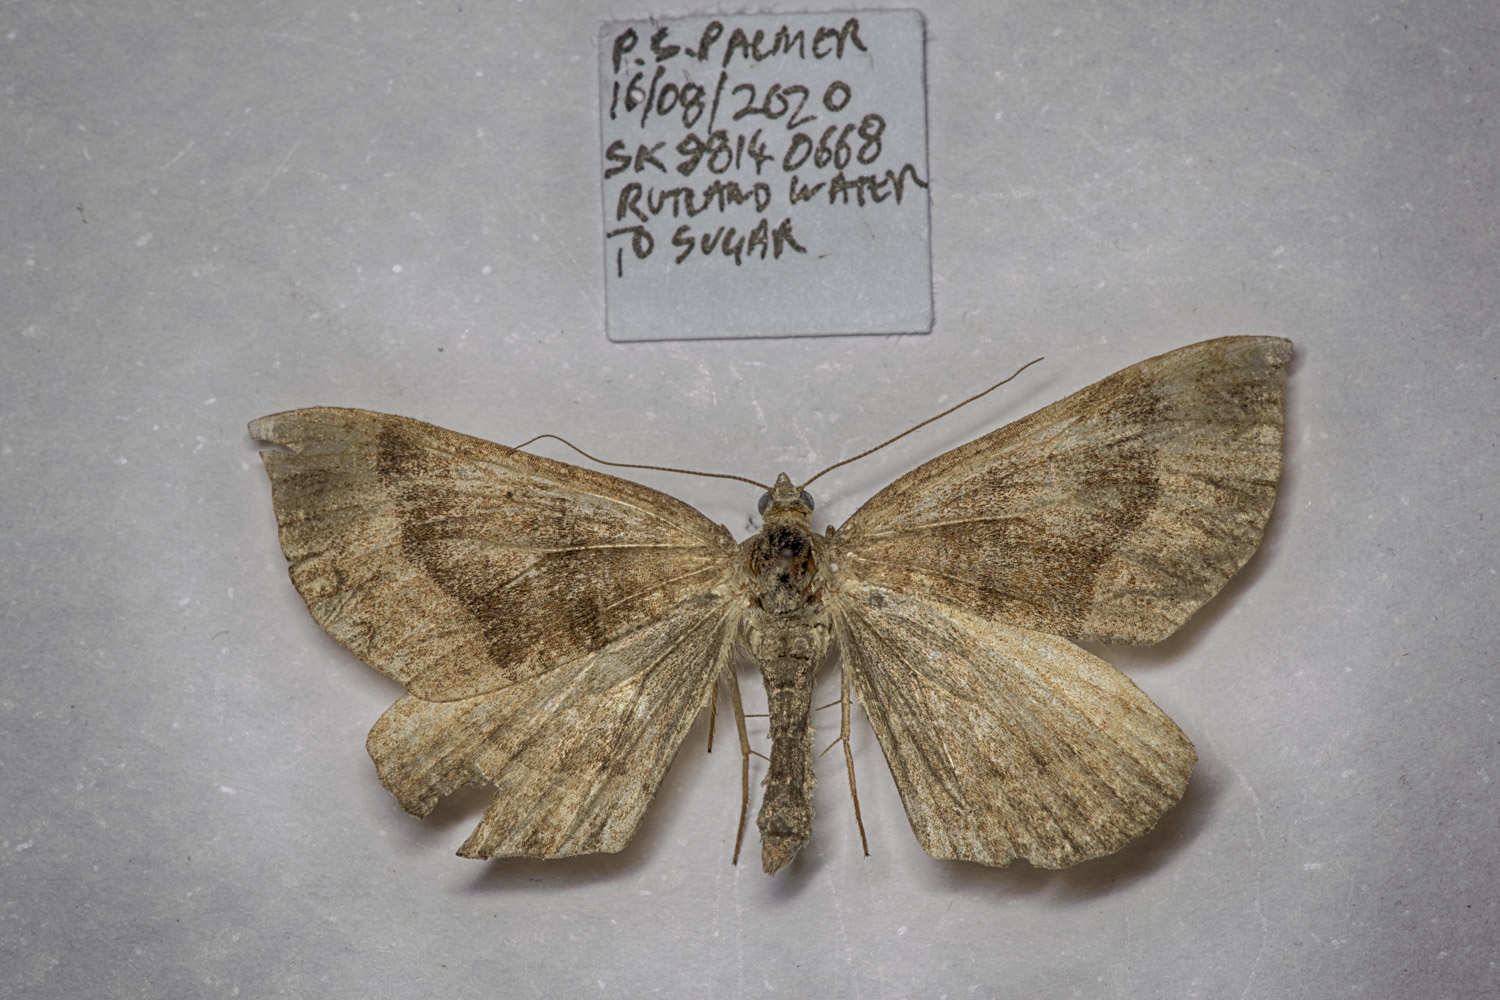
\includegraphics[width=2.14in]{/Users/TechTrends/Documents/my_github/Packages/bookdown-report/_records/dummy-records-delete/dummy/images/202009131026PJP-1} 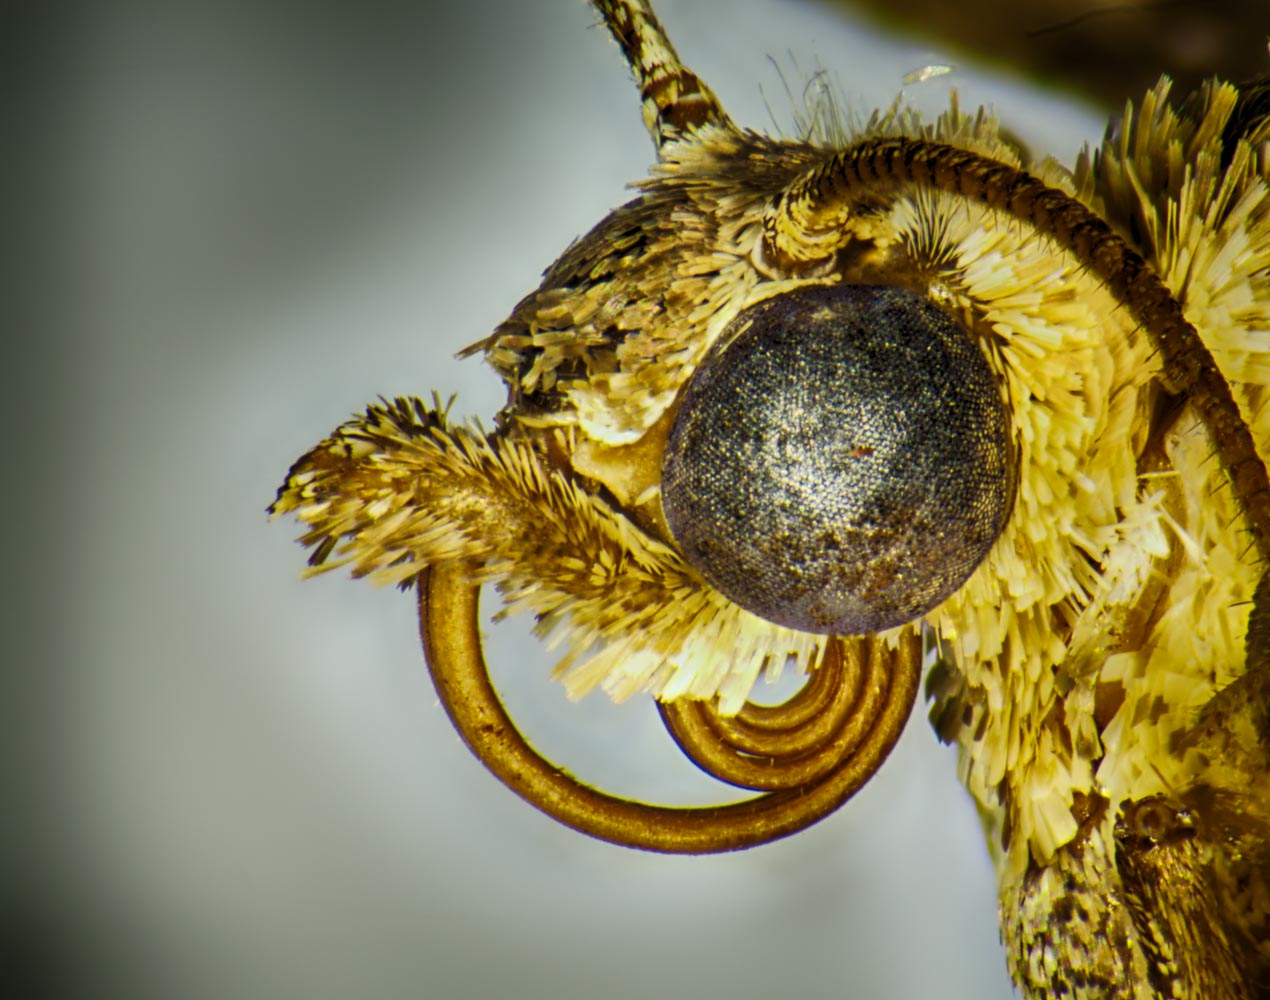
\includegraphics[width=1.81in]{/Users/TechTrends/Documents/my_github/Packages/bookdown-report/_records/dummy-records-delete/dummy/images/20201112-1} 

}

\caption{Specimen images}\label{fig:unnamed-chunk-13}
\end{figure}

\textbf{Observations:} FW.length: Forewing length mm, FW.width: Forewing width mm, EYE.d: Eye diameter mm, Ocelli: Present. Absent, Ocelli.position: Anterior, Posterior, Ocelli.angle: Clockwise angle from antennae, Ocelli.placement: Proximal, Distal, Labial.palps: Upright, Forward, Decending, Frons: Rough, Smooth, Vertex: Rough, Smooth, EYE.texture: Hairy, Hairless, and Chaetosemata: Present, Absent.

\textbf{Dissection:}

\begin{figure}

{\centering 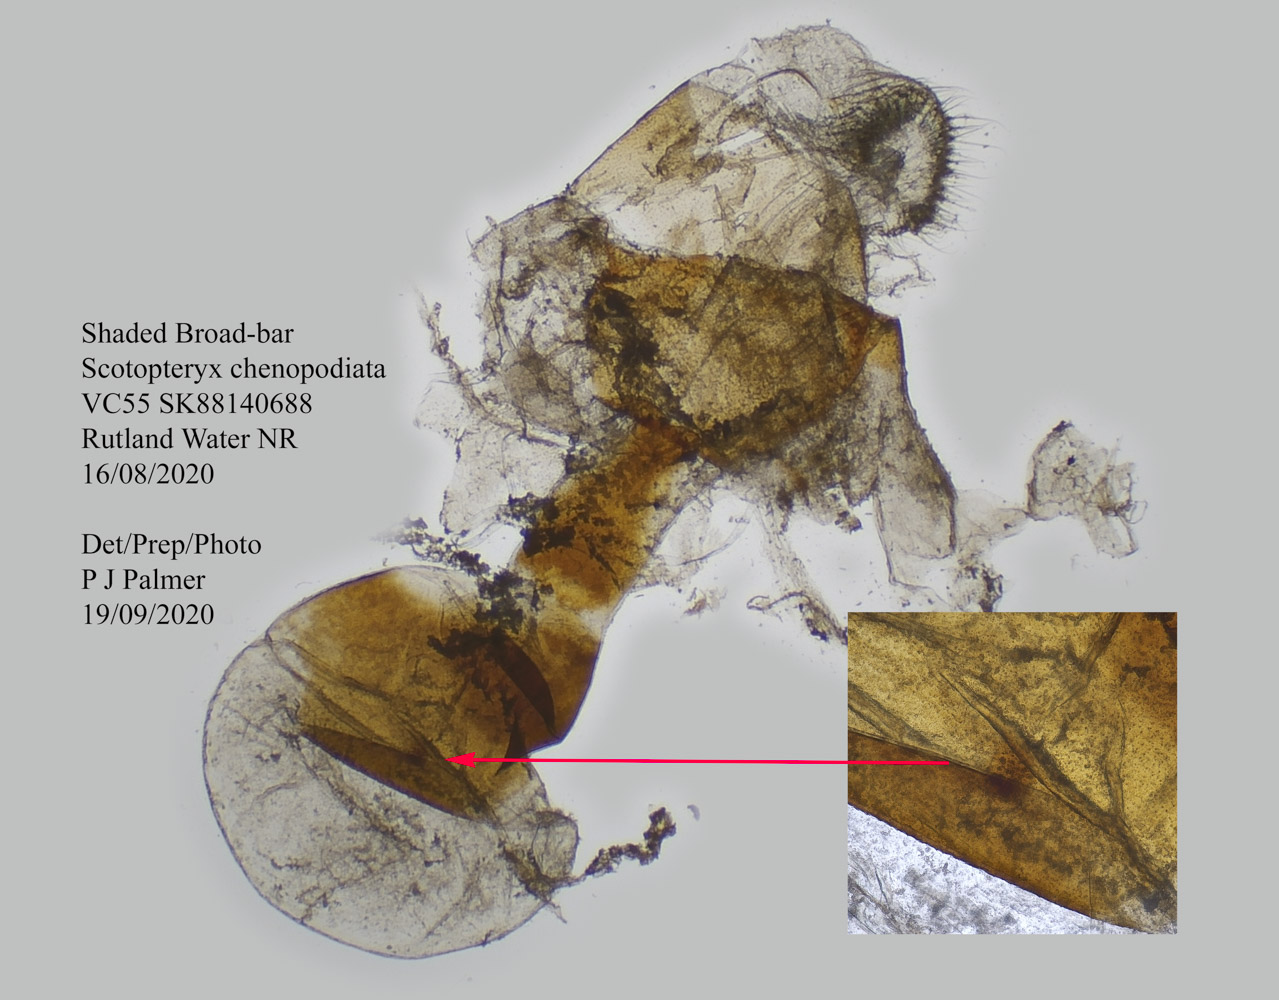
\includegraphics[width=1.83in]{/Users/TechTrends/Documents/my_github/Packages/bookdown-report/_records/dummy-records-delete/dummy/images/dissection/202009131026PJP-3} 

}

\caption{Temporary slide in alcohol gel.}\label{fig:unnamed-chunk-16}
\end{figure}

\begin{Shaded}
\begin{Highlighting}[]
\FunctionTok{library}\NormalTok{(plyr)}
\FunctionTok{library}\NormalTok{(tidyverse)}
\FunctionTok{library}\NormalTok{(ggplot2)}
\FunctionTok{library}\NormalTok{(viridis)}


\NormalTok{absolute.path }\OtherTok{\textless{}{-}}\NormalTok{ rprojroot}\SpecialCharTok{::}\FunctionTok{find\_rstudio\_root\_file}\NormalTok{()}
\CommentTok{\#CountyBoundary \textless{}{-} External[[2]]}
\NormalTok{path.to.VC55 }\OtherTok{\textless{}{-}}\NormalTok{ fs}\SpecialCharTok{::}\FunctionTok{path}\NormalTok{(absolute.path, }\StringTok{"data{-}ext"}\NormalTok{,}\StringTok{"VC55"}\NormalTok{, }\AttributeTok{ext =} \StringTok{"rds"}\NormalTok{)}

\NormalTok{CountyBoundary }\OtherTok{\textless{}{-}} \FunctionTok{readRDS}\NormalTok{(path.to.VC55)}
\CommentTok{\# Set the ESPG}
\CommentTok{\#CountyBoundary \textless{}{-} sf::st\_set\_crs(CountyBoundary, 4326)}
\CommentTok{\# Reproject}
\CommentTok{\# Reproject as UKNG EPSG }
\NormalTok{CountyBoundary }\OtherTok{\textless{}{-}}\NormalTok{ sf}\SpecialCharTok{::}\FunctionTok{st\_transform}\NormalTok{(CountyBoundary, }\DecValTok{27700}\NormalTok{)}
\end{Highlighting}
\end{Shaded}

\begin{Shaded}
\begin{Highlighting}[]
\CommentTok{\# Load the data}
\NormalTok{path.to.my.data }\OtherTok{\textless{}{-}}\NormalTok{ fs}\SpecialCharTok{::}\FunctionTok{path}\NormalTok{( absolute.path}
\NormalTok{                               ,}\StringTok{"data{-}ss"}\NormalTok{,}\StringTok{"data{-}ss"}\NormalTok{, }\AttributeTok{ext =} \StringTok{"rds"}\NormalTok{)}

\NormalTok{my.data.ss }\OtherTok{\textless{}{-}} \FunctionTok{readRDS}\NormalTok{(path.to.my.data)}


\CommentTok{\# Rough check for sensible Grid reference format}
\NormalTok{data.for.spatial }\OtherTok{\textless{}{-}}\NormalTok{ my.data.ss}\SpecialCharTok{$}\NormalTok{grid.ref}

\NormalTok{      rows.with.GR }\OtherTok{\textless{}{-}} \FunctionTok{grepl}\NormalTok{(}\StringTok{"([A{-}Z]\{2\})(}\SpecialCharTok{\textbackslash{}\textbackslash{}}\StringTok{d\{4\}|}\SpecialCharTok{\textbackslash{}\textbackslash{}}\StringTok{d\{6\}|}\SpecialCharTok{\textbackslash{}\textbackslash{}}\StringTok{d\{8\}|}\SpecialCharTok{\textbackslash{}\textbackslash{}}\StringTok{d\{10\})$"}\NormalTok{,data.for.spatial )}

\NormalTok{   rows.to.keep }\OtherTok{\textless{}{-}} \FunctionTok{which}\NormalTok{(rows.with.GR)  }

\NormalTok{   my.data.ss }\OtherTok{\textless{}{-}}\NormalTok{my.data.ss[rows.to.keep,]}
   
   

\NormalTok{my.data.geo }\OtherTok{\textless{}{-}}\NormalTok{ eco.atlas}\SpecialCharTok{::}\FunctionTok{GBNG.to.Lat.Long}\NormalTok{(my.data.ss}\SpecialCharTok{$}\NormalTok{grid.ref)}
\end{Highlighting}
\end{Shaded}

\begin{verbatim}
## Warning in showSRID(uprojargs, format = "PROJ", multiline = "NO", prefer_proj =
## prefer_proj): Discarded datum OSGB_1936 in Proj4 definition
\end{verbatim}

\begin{Shaded}
\begin{Highlighting}[]
\NormalTok{my.dates }\OtherTok{\textless{}{-}}\NormalTok{ eco.atlas}\SpecialCharTok{::}\FunctionTok{Clean.dates}\NormalTok{(my.data.ss}\SpecialCharTok{$}\NormalTok{record.date)}

\NormalTok{working.data }\OtherTok{\textless{}{-}} \FunctionTok{cbind}\NormalTok{(my.data.ss, my.dates, my.data.geo )}

\NormalTok{all.data.df.sf }\OtherTok{\textless{}{-}}\NormalTok{ sf}\SpecialCharTok{::}\FunctionTok{st\_as\_sf}\NormalTok{(working.data, }\AttributeTok{coords=} \FunctionTok{c}\NormalTok{(}\StringTok{"Long"}\NormalTok{,}\StringTok{"Lat"}\NormalTok{))}

\CommentTok{\# Set EPSG 4326 WSG84 as this is the source data}
\NormalTok{all.data.df.sf }\OtherTok{\textless{}{-}}\NormalTok{ sf}\SpecialCharTok{::}\FunctionTok{st\_set\_crs}\NormalTok{(all.data.df.sf, }\DecValTok{4326}\NormalTok{)}

\CommentTok{\# Reproject as UKNG EPSG }
\NormalTok{all.data.df.sf }\OtherTok{\textless{}{-}}\NormalTok{ sf}\SpecialCharTok{::}\FunctionTok{st\_transform}\NormalTok{(all.data.df.sf, }\DecValTok{27700}\NormalTok{)}

\CommentTok{\# Now we have data as UKNG we can work out tetrads}

\NormalTok{coordinates.of.records }\OtherTok{\textless{}{-}}\NormalTok{ sf}\SpecialCharTok{::}\FunctionTok{st\_coordinates}\NormalTok{(all.data.df.sf)}

\NormalTok{coordinates.of.records}\FloatTok{.2}\NormalTok{k }\OtherTok{\textless{}{-}} \FunctionTok{trunc}\NormalTok{(coordinates.of.records}\SpecialCharTok{/} \DecValTok{2000}\NormalTok{) }\SpecialCharTok{*}\DecValTok{2000}
\FunctionTok{colnames}\NormalTok{(coordinates.of.records}\FloatTok{.2}\NormalTok{k) }\OtherTok{\textless{}{-}} \FunctionTok{c}\NormalTok{(}\StringTok{"X.2k"}\NormalTok{, }\StringTok{"Y.2k"}\NormalTok{)}
\NormalTok{all.data.df.sf }\OtherTok{\textless{}{-}} \FunctionTok{cbind}\NormalTok{(all.data.df.sf, coordinates.of.records}\FloatTok{.2}\NormalTok{k)}
\CommentTok{\# Add coordinates as eastings and northings}
\NormalTok{coords.east.north }\OtherTok{\textless{}{-}}\NormalTok{ coordinates.of.records}
\FunctionTok{colnames}\NormalTok{(coords.east.north) }\OtherTok{\textless{}{-}} \FunctionTok{c}\NormalTok{(}\StringTok{"easting"}\NormalTok{, }\StringTok{"northing"}\NormalTok{)}
\NormalTok{all.data.df.sf }\OtherTok{\textless{}{-}} \FunctionTok{cbind}\NormalTok{(all.data.df.sf, coords.east.north)}

\CommentTok{\# Crop data}

\NormalTok{working.data }\OtherTok{\textless{}{-}}\NormalTok{ sf}\SpecialCharTok{::}\FunctionTok{st\_crop}\NormalTok{(all.data.df.sf, CountyBoundary)}
\end{Highlighting}
\end{Shaded}

\begin{verbatim}
## Warning: attribute variables are assumed to be spatially constant throughout all
## geometries
\end{verbatim}

\begin{Shaded}
\begin{Highlighting}[]
\CommentTok{\#working.data \textless{}{-} all.data.df.sf}
\NormalTok{gplot1 }\OtherTok{\textless{}{-}} \FunctionTok{ggplot}\NormalTok{()  }\SpecialCharTok{+} 
 \FunctionTok{geom\_sf}\NormalTok{(}\AttributeTok{data =}\NormalTok{CountyBoundary ) }\SpecialCharTok{+}
  \FunctionTok{geom\_bin2d}\NormalTok{( }\AttributeTok{data =}\NormalTok{ working.data, }
              \AttributeTok{binwidth =} \FunctionTok{c}\NormalTok{(}\DecValTok{2000}\NormalTok{,}\DecValTok{2000}\NormalTok{), }
              \FunctionTok{aes}\NormalTok{(}\AttributeTok{x=}\NormalTok{easting, }\AttributeTok{y=}\NormalTok{northing)) }\SpecialCharTok{+} 
              \FunctionTok{coord\_sf}\NormalTok{(}\AttributeTok{crs =} \DecValTok{27700}\NormalTok{) }\SpecialCharTok{+}  
              \FunctionTok{scale\_fill\_viridis}\NormalTok{(}\AttributeTok{trans =} \StringTok{"log10"}\NormalTok{)}

\NormalTok{gplot1}
\end{Highlighting}
\end{Shaded}

\begin{figure}

{\centering \includegraphics{_main_files/figure-latex/unnamed-chunk-6-1} 

}

\caption{Map of all records by tetrad.}\label{fig:unnamed-chunk-6}
\end{figure}

\begin{Shaded}
\begin{Highlighting}[]
\CommentTok{\# Create factor of included years}
\NormalTok{YYYY.factor }\OtherTok{\textless{}{-}}\NormalTok{ working.data}\SpecialCharTok{$}\NormalTok{YYYY }\SpecialCharTok{\%\textgreater{}\%} \FunctionTok{unique}\NormalTok{() }\SpecialCharTok{\%\textgreater{}\%} \FunctionTok{as.character}\NormalTok{() }\SpecialCharTok{\%\textgreater{}\%} \FunctionTok{fct\_inseq}\NormalTok{()}
\NormalTok{MM.factor }\OtherTok{\textless{}{-}} \FunctionTok{c}\NormalTok{(}\StringTok{"01"}\NormalTok{,}\StringTok{"02"}\NormalTok{,}\StringTok{"03"}\NormalTok{,}\StringTok{"04"}\NormalTok{,}\StringTok{"05"}\NormalTok{,}\StringTok{"06"}\NormalTok{,}\StringTok{"07"}\NormalTok{,}\StringTok{"08"}\NormalTok{,}\StringTok{"09"}\NormalTok{,}\StringTok{"10"}\NormalTok{,}\StringTok{"11"}\NormalTok{,}\StringTok{"12"}\NormalTok{)}

\NormalTok{working.data}\SpecialCharTok{$}\NormalTok{count }\OtherTok{\textless{}{-}} \DecValTok{1}
\NormalTok{temp.data.ag.by.month }\OtherTok{=} \FunctionTok{aggregate}\NormalTok{(count }\SpecialCharTok{\textasciitilde{}}\NormalTok{ YYYY }\SpecialCharTok{+}\NormalTok{ MM, }
                                         \AttributeTok{data=}\NormalTok{working.data, sum, }\AttributeTok{na.rm=}\ConstantTok{TRUE}\NormalTok{)}
\CommentTok{\# Add missing factor levels}

\NormalTok{temp.data.ag.by.month}\SpecialCharTok{$}\NormalTok{YYYY }\OtherTok{\textless{}{-}} \FunctionTok{factor}\NormalTok{(temp.data.ag.by.month}\SpecialCharTok{$}\NormalTok{YYYY, YYYY.factor) }\SpecialCharTok{\%\textgreater{}\%} \FunctionTok{fct\_inseq}\NormalTok{()}
\CommentTok{\# Addd missing factor values}
\NormalTok{temp.data.ag.by.month}\SpecialCharTok{$}\NormalTok{MM }\OtherTok{\textless{}{-}} \FunctionTok{factor}\NormalTok{(temp.data.ag.by.month}\SpecialCharTok{$}\NormalTok{MM, }
  \AttributeTok{levels =}\NormalTok{ MM.factor )}

\CommentTok{\# temp.data.ag.by.month.all$MM \textless{}{-} temp.data.ag.by.month.all$MM \%\textgreater{}\% as.numeric()}
\CommentTok{\# temp.data.ag.by.month.all \textless{}{-} temp.data.ag.by.month.all[order(temp.data.ag.by.month.all$MM),]}


\NormalTok{gplotStrip }\OtherTok{\textless{}{-}} \FunctionTok{ggplot}\NormalTok{(}\AttributeTok{data =}\NormalTok{ temp.data.ag.by.month)  }\SpecialCharTok{+}
    \FunctionTok{ggtitle}\NormalTok{(}\StringTok{"Records by month"}\NormalTok{) }\SpecialCharTok{+}
  \FunctionTok{geom\_tile}\NormalTok{( }
                      \FunctionTok{aes}\NormalTok{(}\AttributeTok{x=}\NormalTok{YYYY,}\AttributeTok{y=}\NormalTok{MM, }\AttributeTok{fill=}\NormalTok{ count))  }\SpecialCharTok{+}
   \FunctionTok{scale\_y\_discrete}\NormalTok{(}\AttributeTok{drop =} \ConstantTok{FALSE}\NormalTok{) }\SpecialCharTok{+} 
  \FunctionTok{scale\_x\_discrete}\NormalTok{(}\AttributeTok{drop =} \ConstantTok{FALSE}\NormalTok{) }\SpecialCharTok{+} 
  \FunctionTok{scale\_fill\_viridis}\NormalTok{( }\AttributeTok{discrete =} \ConstantTok{FALSE}\NormalTok{, }\AttributeTok{trans =} \StringTok{"log10"}\NormalTok{, }\AttributeTok{option =} \StringTok{"A"}\NormalTok{) }\SpecialCharTok{+} 
  \FunctionTok{theme\_minimal}\NormalTok{() }\SpecialCharTok{+}  \FunctionTok{coord\_fixed}\NormalTok{() }\SpecialCharTok{+}
  \FunctionTok{theme}\NormalTok{(}\AttributeTok{axis.text.x  =} \FunctionTok{element\_text}\NormalTok{(}\AttributeTok{angle=}\DecValTok{45}\NormalTok{, }\AttributeTok{hjust =} \DecValTok{1}\NormalTok{),}
        \AttributeTok{axis.title =} \FunctionTok{element\_blank}\NormalTok{())}

\CommentTok{\#grid.arrange(gplot1, gplot3, nrow = 1)}

\CommentTok{\#grid.arrange(gplot1, gplotpost, gplotStrip, nrow = 2)}
\NormalTok{lay }\OtherTok{\textless{}{-}} \FunctionTok{rbind}\NormalTok{(}\FunctionTok{c}\NormalTok{(}\DecValTok{1}\NormalTok{,}\DecValTok{2}\NormalTok{),}
             \FunctionTok{c}\NormalTok{(}\DecValTok{3}\NormalTok{,}\DecValTok{3}\NormalTok{))}

\CommentTok{\#grid.arrange(gplot1,  gplotStrip, layout\_matrix = lay)}

\NormalTok{gplotStrip}
\end{Highlighting}
\end{Shaded}

\begin{figure}

{\centering \includegraphics{_main_files/figure-latex/unnamed-chunk-7-1} 

}

\caption{Phenology of all records.}\label{fig:unnamed-chunk-7}
\end{figure}

\hypertarget{introduction}{%
\section{Introduction}\label{introduction}}

This report records the determinations made by microscopic examination of Lepidoptera specimens made by VC55 recorders. Specimens were not retained, as each determination is illustrated by micro-photographs of specimens and temporary slides. The high quality micro-photographs were produced by stacked focus photography and are much easier to work with than traditional permanent slides. In most cases, the artificial depth of field provides a better view of dissected parts than can be seen through a microscope. Using micro-photographs has also allowed on-line collaboration using the version management tool GitHub (\url{https://github.com}) to manage this and other reports.

The primary sources for identifying Lepidoptera by dissection used in this work are @Hall2021 and @Schon2021. The determination was also checked against the appearance of the imago using @Kimber2021 amongst other sources.

\hypertarget{species-summary}{%
\section{Species Summary}\label{species-summary}}

The species recorded are presented in Table \ref{tab:TableSpeciesList} which has been directly generated from the records.

\begin{table}

\caption{\label{tab:TableSpeciesList}Species recorded by family and gender.}
\centering
\begin{tabular}[t]{lllr}
\toprule
family & taxon & gender & Count\\
\midrule
\cellcolor{gray!6}{Dummida} & \cellcolor{gray!6}{Funny} & \cellcolor{gray!6}{Male, Female} & \cellcolor{gray!6}{1}\\
\bottomrule
\end{tabular}
\end{table}

A total of 1 specimens were examined of which 1 were identified.

\begin{figure}[p]

{\centering \includegraphics{_main_files/figure-latex/unnamed-chunk-23-1} 

}

\caption{Map of all records by tetrad.}\label{fig:unnamed-chunk-23}
\end{figure}

\begin{figure}[p]

{\centering \includegraphics{_main_files/figure-latex/unnamed-chunk-24-1} 

}

\caption{Phenology of all records.}\label{fig:unnamed-chunk-24}
\end{figure}

\hypertarget{dummy-records-1}{%
\section{Dummy Records}\label{dummy-records-1}}

This is a collation of all Dummy records from the \textbf{\_records} directory which comprises the source documents for all the ID sheets.

\hypertarget{specimen-dummy-funny-common-name-1}{%
\subsection*{Specimen dummy Funny Common Name}\label{specimen-dummy-funny-common-name-1}}
\addcontentsline{toc}{subsection}{Specimen dummy Funny Common Name}

\textbf{Label details}:
record.date: 2021-09-01, place.name: Garden, grid.ref: SK75651803, recorder.name: Recorder, record.notes: Notes, determiner: Determiner, order: Dummy, family: Dummida, sub.family: Dummissiae, genus: Dummidus, taxon: Funny, log.number: Classification Log Number, Bradley: Bradley Fletcher Number, common.name: Common Name, and gender: Male, Female.

\begin{figure}[p]

{\centering 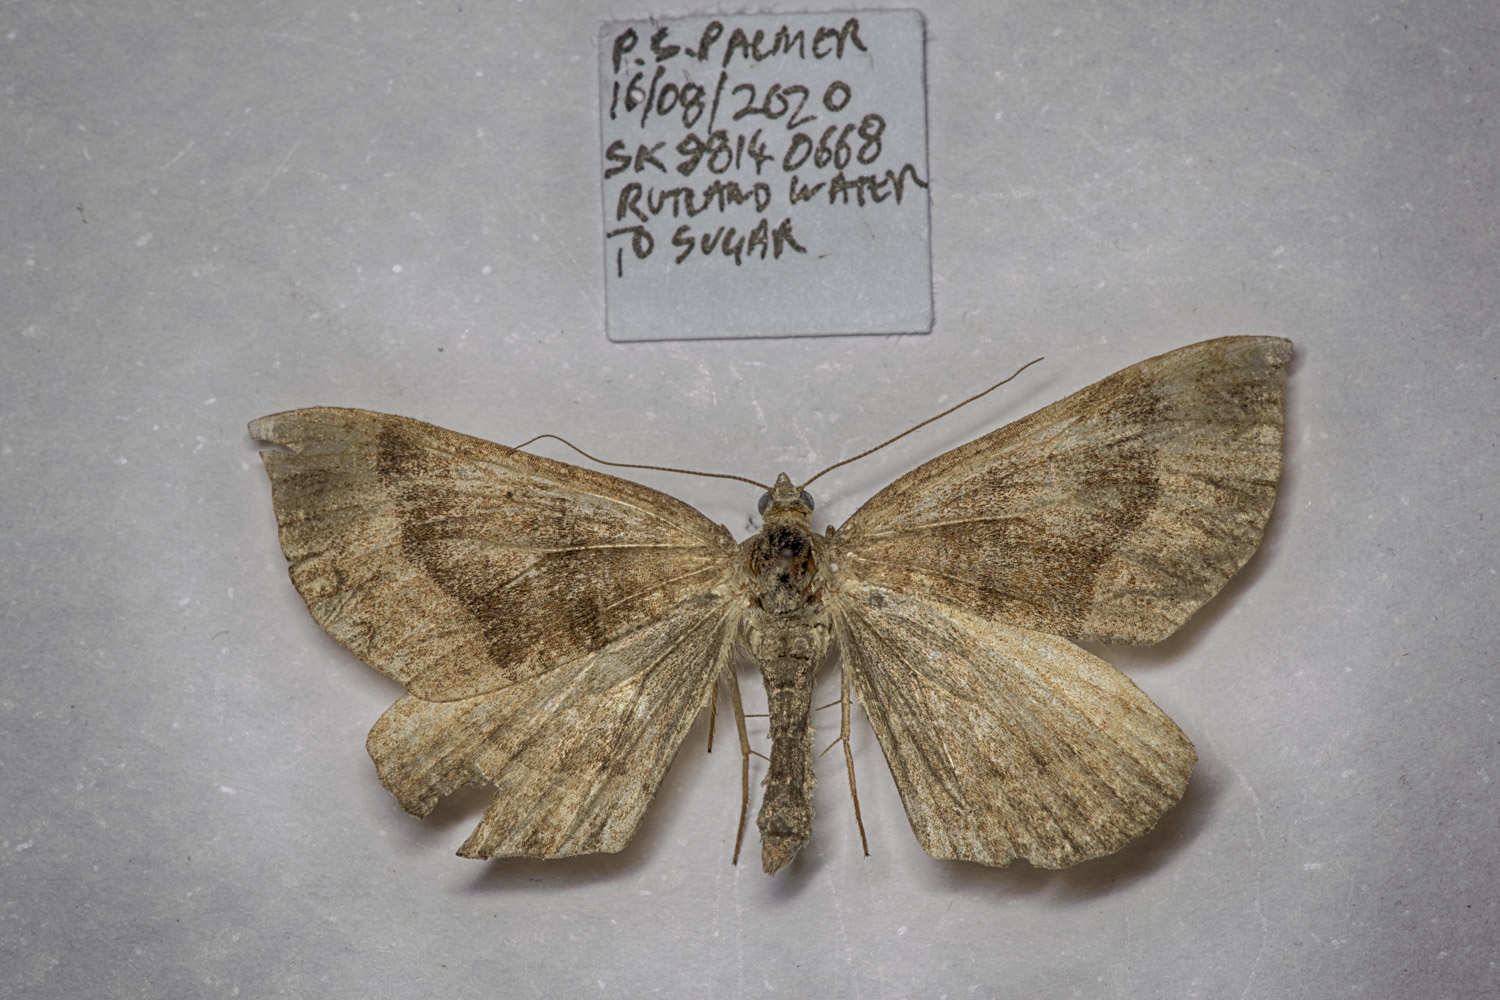
\includegraphics[width=2.14in]{/Users/TechTrends/Documents/my_github/Packages/bookdown-report/_records/dummy-records-delete/dummy/images/202009131026PJP-1} 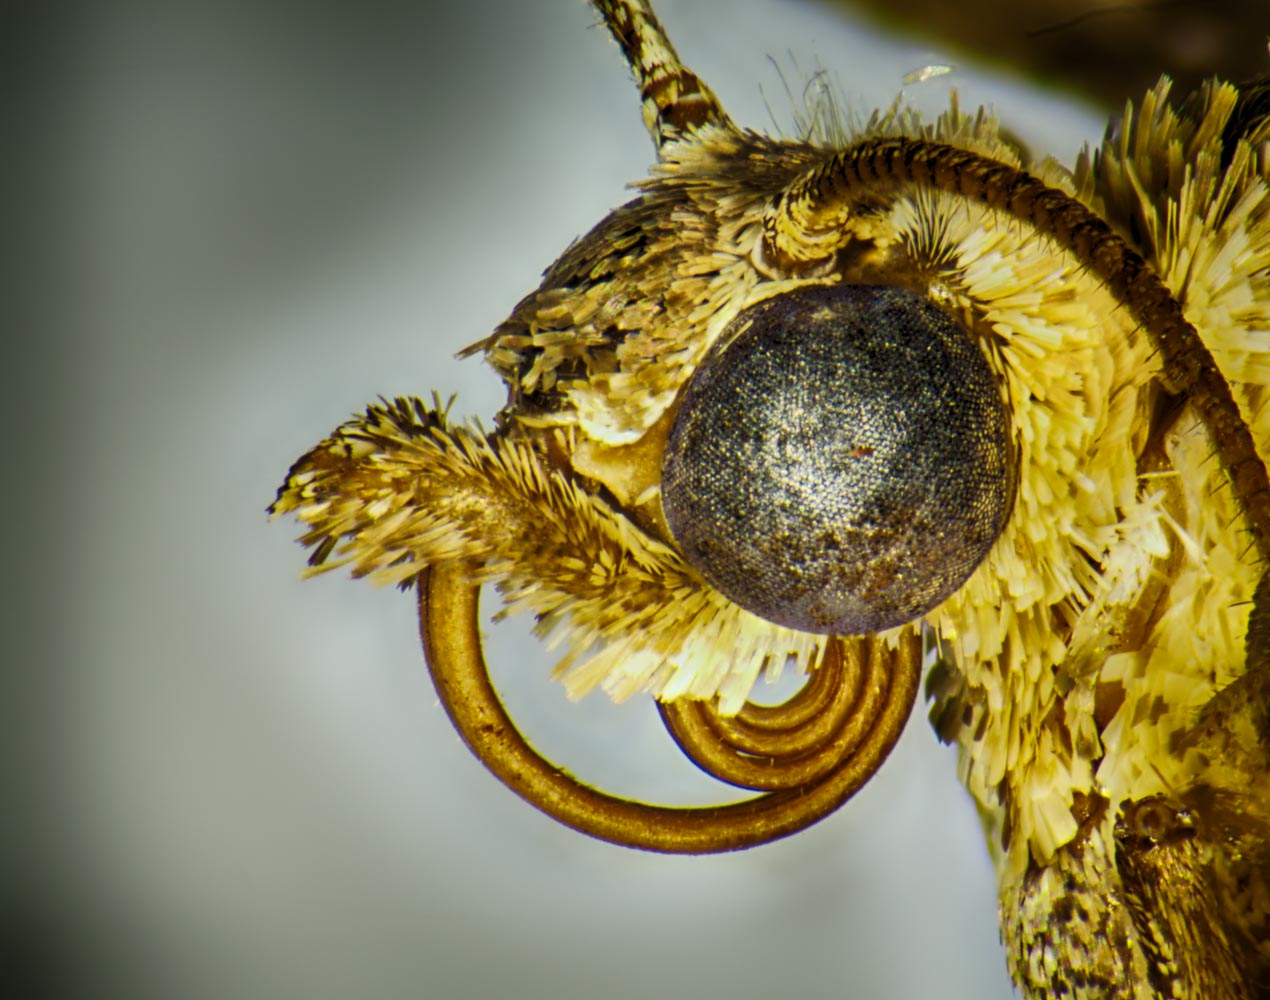
\includegraphics[width=1.81in]{/Users/TechTrends/Documents/my_github/Packages/bookdown-report/_records/dummy-records-delete/dummy/images/20201112-1} 

}

\caption{Specimen images}\label{fig:unnamed-chunk-31}
\end{figure}

\textbf{Observations:} FW.length: Forewing length mm, FW.width: Forewing width mm, EYE.d: Eye diameter mm, Ocelli: Present. Absent, Ocelli.position: Anterior, Posterior, Ocelli.angle: Clockwise angle from antennae, Ocelli.placement: Proximal, Distal, Labial.palps: Upright, Forward, Decending, Frons: Rough, Smooth, Vertex: Rough, Smooth, EYE.texture: Hairy, Hairless, and Chaetosemata: Present, Absent.

\textbf{Dissection:}

\begin{figure}[p]

{\centering 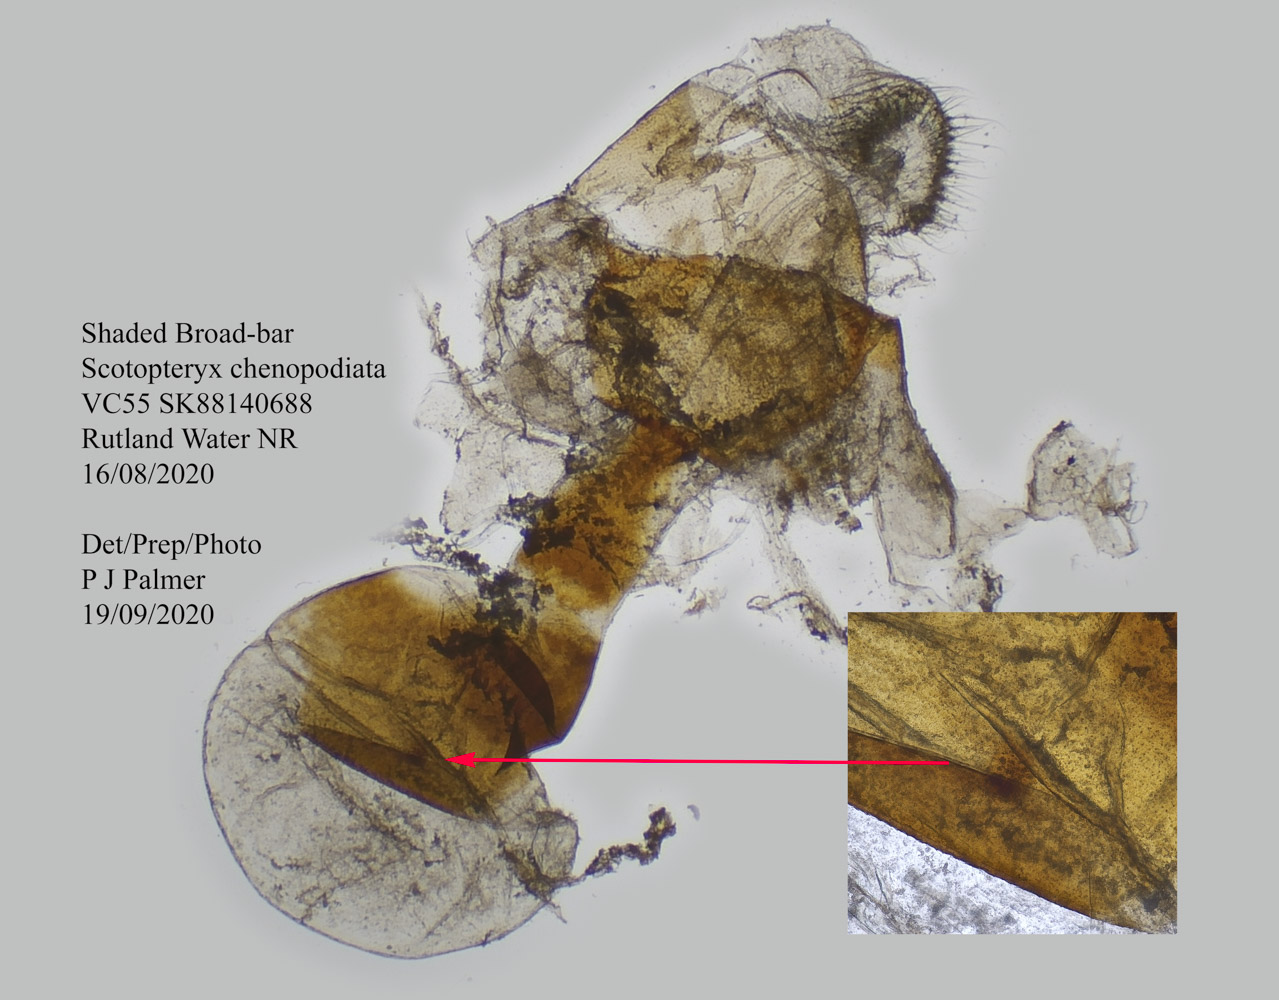
\includegraphics[width=1.83in]{/Users/TechTrends/Documents/my_github/Packages/bookdown-report/_records/dummy-records-delete/dummy/images/dissection/202009131026PJP-3} 

}

\caption{Temporary slide in alcohol gel.}\label{fig:unnamed-chunk-34}
\end{figure}

\hypertarget{references}{%
\section*{References}\label{references}}
\addcontentsline{toc}{section}{References}

\hypertarget{refs}{}
\begin{CSLReferences}{0}{0}
\end{CSLReferences}

\let\cleardoublepage\clearpage

\end{document}
